\label{DL_theory}
\section{Deep Learning for spectroscopic data}

Techniques of machine learning and deep learning specifically have been applied to spectroscopic data since the 1990s. It has been applied to a variety of spectroscopic methods such as Near Infrared Spectroscopy (NIR), Raman Spectroscopy, Nuclear Magnetic Resonance Spectroscopy (NMR) and Infrared Spectroscopy (IR) . However, chemometric or physics-based approaches have been and still are favored for data analysis due to the lack of model explainability for data-driven approaches. To oppose, chemometrics is most often based on decomposition techniques such as Principal Component Analysis (PCA) and subsequent linear regression - which inherently does not meet the requirements for explainability.


% advances in DL & applications to spectroscopy tasks
\subsection{General patterns}

\subsubsection{Dense layers}
What is often referred to as fully connected, dense, or feedforward neural network describes a network consisting of solely densely connected layers. These layers are connected in an $n:m$ manner, where each node of layer with n nodes is connected with each node of layer with m nodes.


\subsubsection{Dropout}
Dropout layers are often used to regularize and generalize models. In these layers, which are fully connected layers, a certain percentage of nodes are not used during training and the specific unused nodes are selected from new each time.

\subsubsection{}

\subsection{Convolutional Neural Networks (CNN)}

In convolutional neural networks (CNN), the input values are multiplied with a kernel to extract features. The CNNs are used where the input is of a discrete, grid-like topology. A kernel in this sense can represent a vector of n dimensions, where in case of spectra n=1 that will be moved along an axis, applying the multiplication subsequently. The values of the kernel are learnable, such that it can be fitted to extract specific features depending on the nature of the data.

These convolutional layers are usually followed by pooling layers - such as max-pooling or average-pooling - which also use a kernel. As the pooling layers reduce the dimensionality of the input, they have a number of positive effects on the model, such as better robustness to input variability and faster training. In addition, pooling layers help the model to learn invariances in the input data, such as rotation of an image. 

The 1-dimensional convolutions we use in the case of spectral data will thus use $p$ one-dimensional kernels (vectors) of pre-defined length, where $p$ stands for the number of channels. If, for example, our spectrum vector is of dimensions (1 x 1024), using a 1d-convolutional kernel of size (1 x 5) with will be applied.

This network architectural pattern is extensively used in image classification tasks but has also been applied to many similar tasks, including spectroscopic data analysis \cite{sun_cnnlstm_2023, castorena_deep_2021, drera_deep_2019}.

\subsection{Residual networks}

In residual networks, the input is re-added after performing convolutional operations. This feature has known positive effects, especially on deeper neural networks (networks with multiple layers). Residual network architectures diminish the well-known vanishing graident problem by re-feeding the network with previous layers. The structure usually involves convolutions of the input before re-adding the input to the 

\begin{figure}
    \centering
    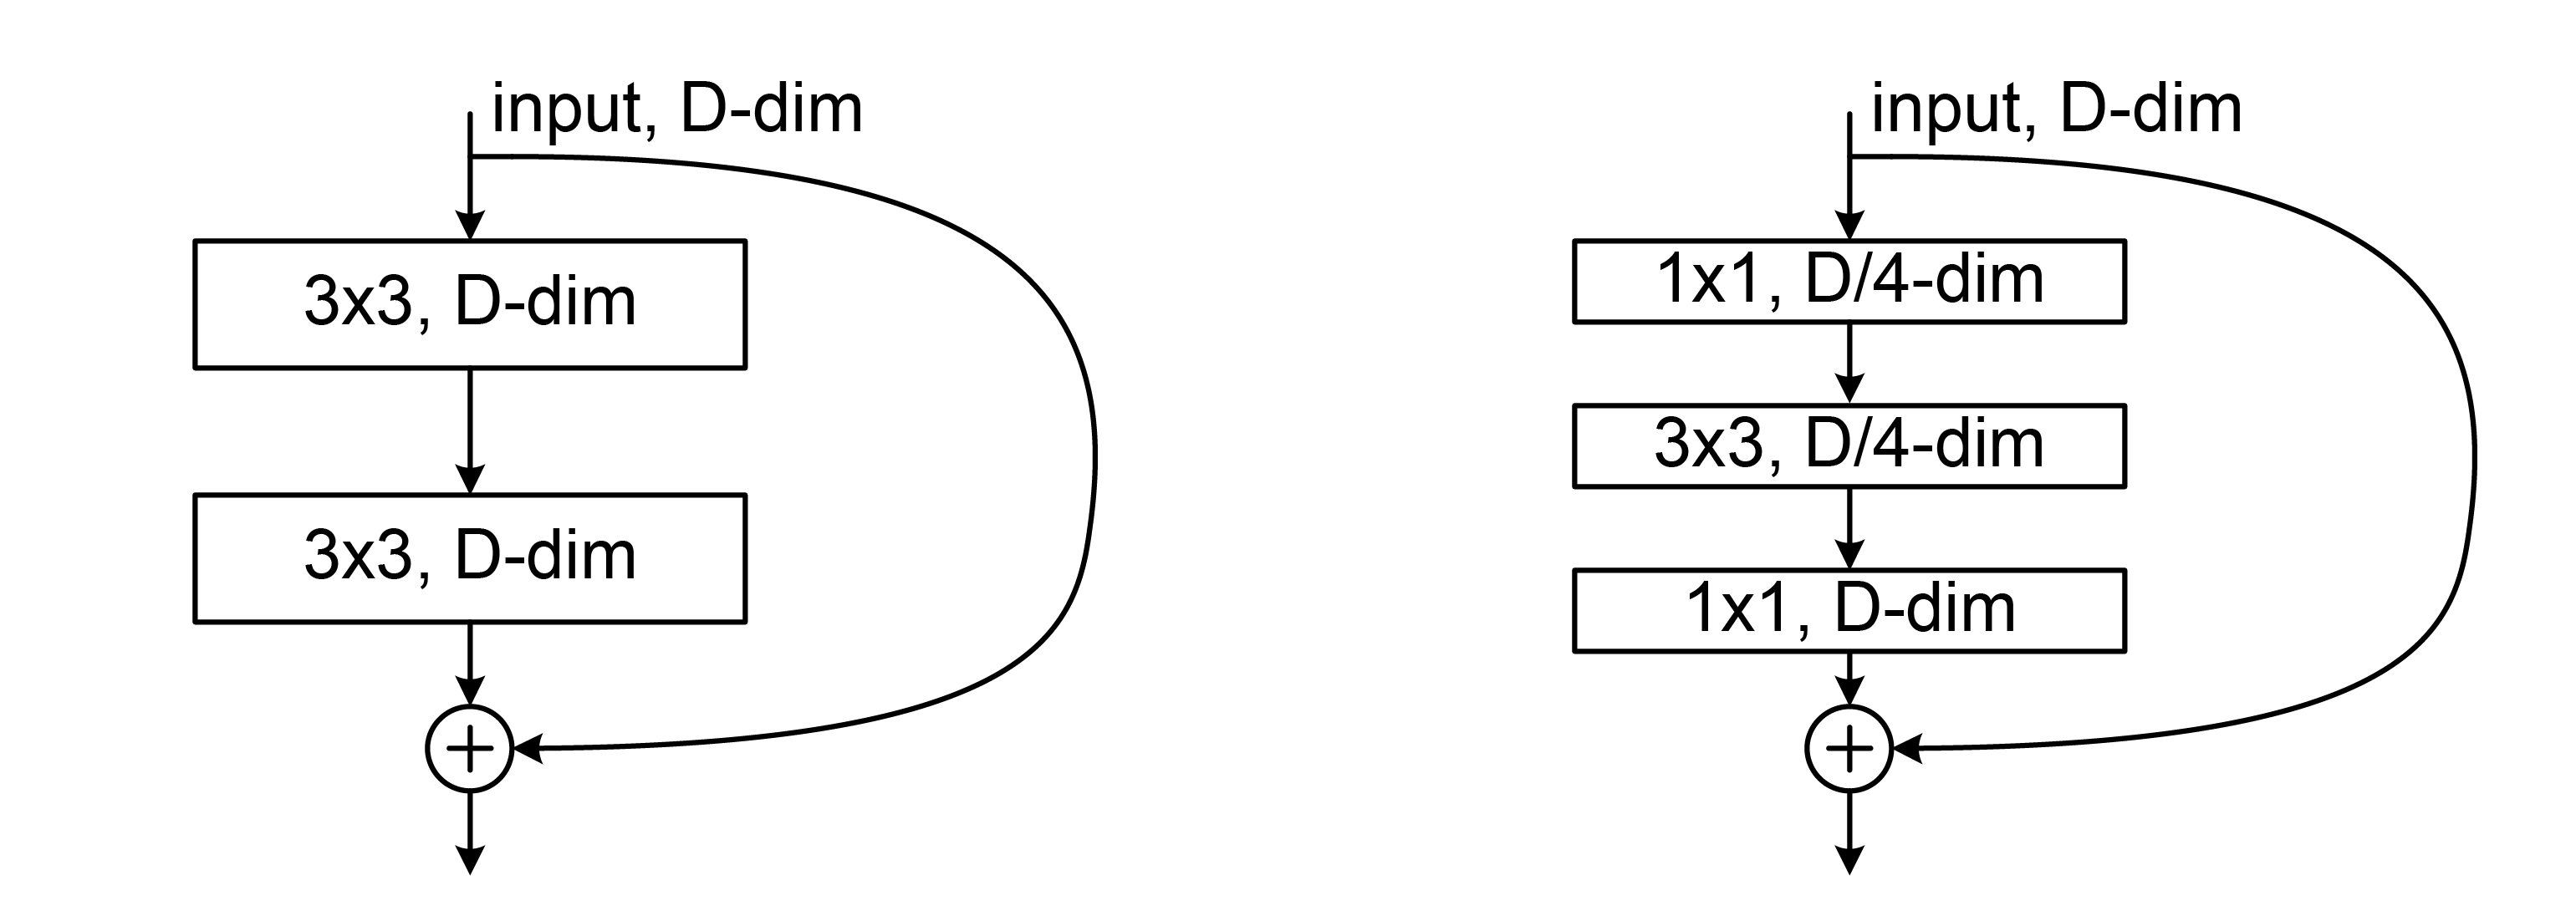
\includegraphics{Figures/ResBlockVariants.png}
    \caption{Residual block pattern}
    \label{fig:res_block}
\end{figure}


\subsection{Recurrent neural networks}

In recurrent neural networks (RNNs), temporal information is kept in a hidden representation vector. Because of this temporal representation, RNNs are specialized for processing sequences

\subsection{Transformer-based networks}

Originally developed to solve neural language processing (NLP) tasks, the attention mechanism was first described in 2017 \cite{vaswani_attention_2023}.
The combination of an encoder-decoder paradigm with the Multi-Head Attention architecture lead to the development of the Transformer model. This is shown in \ref{fig:transformer_model}
A transformer consists of tokenizers, embedding layers and transformer layers which include the Attention layers and Multilayer perceptron layers.

\begin{figure}
    \centering
    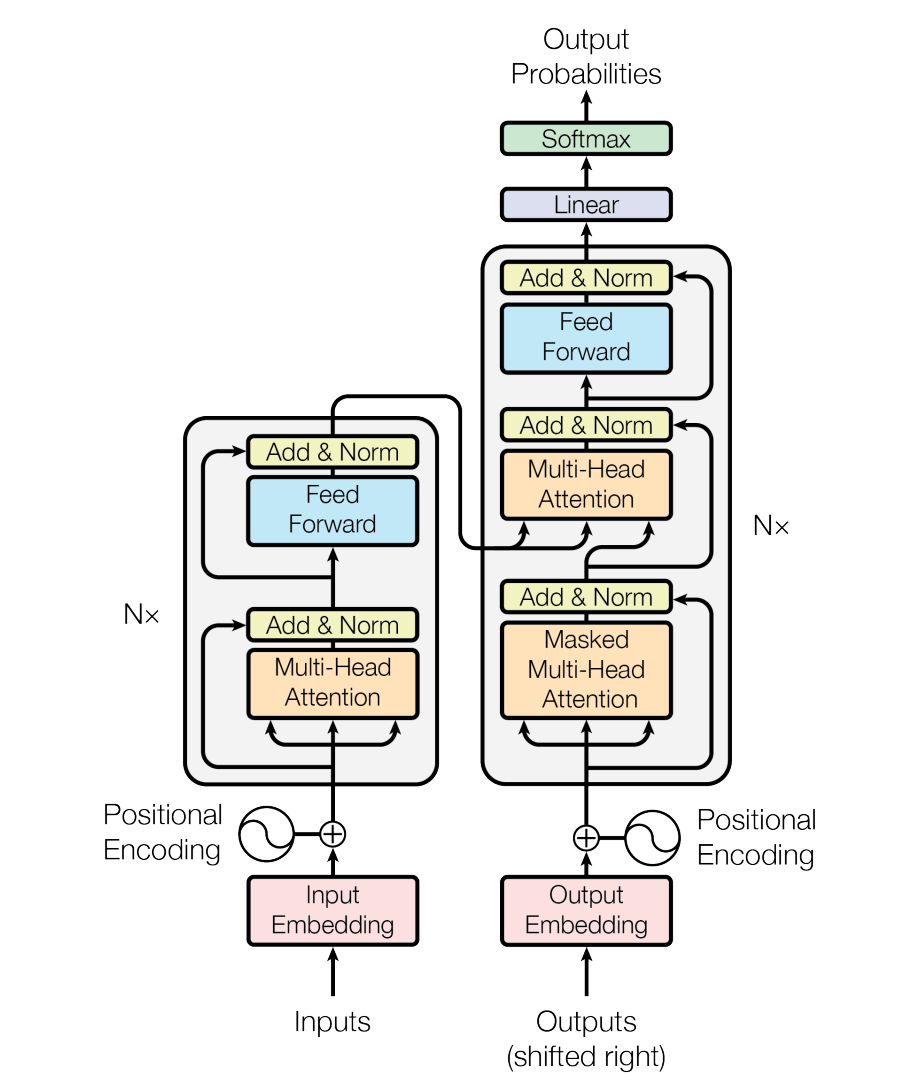
\includegraphics[width=0.6\textwidth]{Figures/Transformer.png}
    \caption{The Transformer-model architecture \cite{vaswani_attention_2023}}
    \label{fig:transformer_model}
\end{figure}

The positional embedding ensures that the model can interpret the position of the tokens within the sequence.

The Multi-Head Attention block consist of linear mappings of query, key and value pairs which are run in parallel. Thus, the attention function is performed on a set of queries and an attention matrix is computed \cite{vaswani_attention_2023}.

\subsubsection{Visual Transformer}

The visual transformer model (ViT) has been recently published \cite{dosovitskiy_image_2021} and uses the mechanisms of Transformer-based models for computer vision tasks. Input data is divided into multiple patches of size n. A positional embedding is added and the embedded patches are then used as tokenized input to the transformer encoder. 


\subsubsection{Visual Attention}